\documentclass[../main.tex]{subfiles}

\begin{document}
	\section{Лекция 8. Двоичные деревья поиска.}
	
	Пусть мы хотим реализовать структуру данных, моделирующую множество. Для этого нам надо уметь быстро \textit{вставлять, искать} и \textit{удалять} элементы из множества. В этом нам поможет такая структура, как \textit{двоичное дерево поиска}.
	
	\subsection{Двоичное дерево поиска}
	 
	\subsubsection{Построение}
	
	Будем называть двоичное дерево $T$ \textit{деревом поиска}, если для него выполняются следующие условия:
	\begin{enumerate}
		\item У любого узла существует не более двух детей
		\item Если узел $y$ лежит в левом поддереве с корнем $x$, то $y.key \leqslant x.key$; если в правом, то $y.key \geqslant x.key$.
	\end{enumerate}

	\begin{remark}
		Строгость неравенства зависит от поставленной задачи. Например, при реализации multiset'а неравенство нестрогое, а при реализиации set'а -- строгое.
	\end{remark}
	
	Приведем пример двоичного дерева поиска:
	
	 \begin{center}
	 	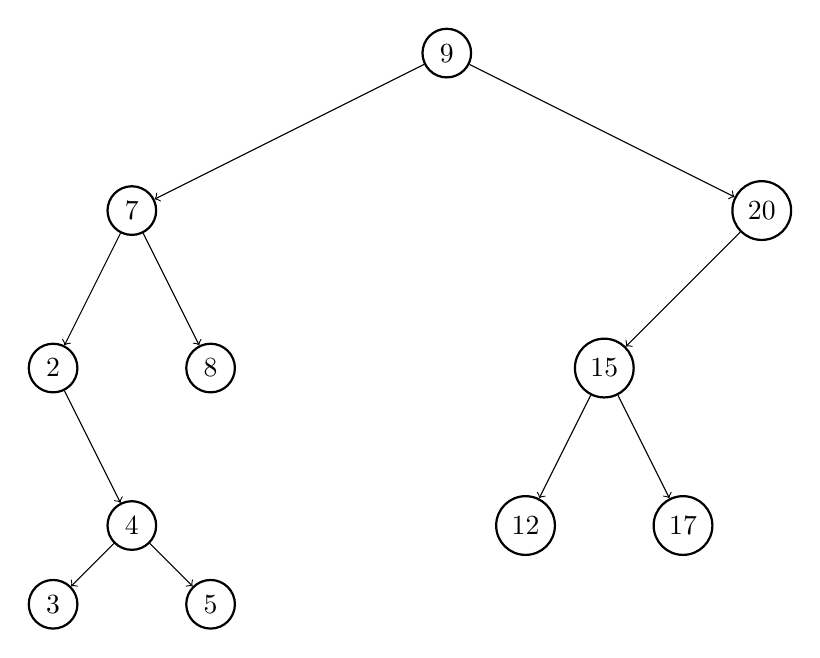
\begin{tikzpicture}
	 	\begin{scope}[every node/.style={circle,thick,draw}]
	 	\node (top) at (10, 10) {$9$};
	
	 	\node (2-1) at (6, 	8) 	{$7$};
	 	\node (2-2) at (14, 8) 	{$20$};
	
	 	\node (3-1) at (5,  6) 	{$2$};
	 	\node (3-2) at (7,  6) 	{$8$};
	 	\node (3-3) at (12, 6)  {$15$};
	
	 	\node (4-2) at (6,  4)	{$4$};
	 	\node (4-3) at (11, 4)	{$12$};
	 	\node (4-4) at (13, 4) 	{$17$};
	
	 	\node (5-1) at (5,  3)  {$3$};
	 	\node (5-2) at (7,  3)  {$5$};
	 	\end{scope}
	
	
	 	\path [->] (top) edge (2-1);
	 	\path [->] (top) edge (2-2);
	
	
	 	\path [->] (2-1) edge (3-1);
	 	\path [->] (2-1) edge (3-2);
	 	\path [->] (2-2) edge (3-3);
	
	 	\path [->] (3-1) edge (4-2);
	 	\path [->] (3-3) edge (4-3);
	 	\path [->] (3-3) edge (4-4);
	
	
	 	\path [->] (4-2) edge (5-1);
	 	\path [->] (4-2) edge (5-2);
	
	 	\end{tikzpicture}
	 \end{center}

	\textit{Весь код в этой лекции будет написан в Python-подобном синтаксисе}	
	
	Для начала опишем поиск в такой структуре:
	\begin{lstlisting}[language=python]
def tree_search(x, k):
    if x:
        if k < x.key:
            return tree_search(x.left, k)
        elif k > x.key:
            return tree_search(x.right, k)
        else:
            return x
    return None
	\end{lstlisting}
	
	Словами: на каждом шаге сравниваем с текущим и идем в нужную ветку.
	
	\begin{time}
		В худшем случае время работы данного алгоритма займет $O(height(T))$, где $T$ -- дерево.
	\end{time}
	
	Затем нужно научиться вставлять ноды в дерево. Основная идея: вставляем в корень, проверяем выполнение инварианта, останавливаемся, если все хорошо, и идем дальше иначе. 
	
	\begin{lstlisting}[language=python]
def tree_insert(t, k): # t -- tree
    z = Node(k)
    x = t.root
    while x:
        z.parent = x
        if z.key > x.key:
            x = x.right
        else:
            x = x.left

    if z.parent:
        if z.key > z.parent.key:
            z.parent.right = z
        else:
            z.parent.left = z
    else:
        t.root = z
	\end{lstlisting}
	
	
	\subsubsection{Сортировка}
	
	Дерево хорошо тем, что если оно у нас уже есть, мы можем за $O(n)$ вывести все элементы по порядку. Идея проста: на каждой ноде сначала выводим правое поддерево, а потом левое поддерево.
	
	\begin{lstlisting}[language=python]
def in_order(x):
    if x.left:
        in_order(x.left)
    print(x.key)
    if x.right:
	    in_order(x.right)
	\end{lstlisting}
	
	Если же дерево не построено, то достаточно легко построить такое дерево и просто вывести:
	
	\begin{lstlisting}[language=python]
def sort(l):
    Tree t
    for key in l:
        tree_insert(t, key)
    in_order(t.root)
	\end{lstlisting}
	
	\begin{remark}
		Сортировка, построенная таким образом эквивалентна алгоритму QuickSort в силу построения дерева: на каждом шаге как будто выбирается \textit{опорный} элемент, относительно которого и происходит разделение массива
	\end{remark}
	
	
	\subsection{Сбалансированное дерево}
	
	\begin{definition}
		\textit{Сбалансированные деревья поиска} -- это такие деревья поиска, что их максимальная высота является $O(\log n)$. Также такие деревья называются \textit{полными} деревьями поиска.
	\end{definition}
	
	Рассмотрим семейство деревьев $\mathcal{F}$, для которых выполняется следующий инвариант:
	\[
	\exists c > 0 \ \forall n \in T: \ |height(n.left) - height(n.right)| \leqslant c
	\]
	
	\begin{theorem}
		Все деревья из $\mathcal{F}$ сбалансированны.
	\end{theorem}
	\begin{proof}
		Пусть $n(h)$ -- минимально возможное число узлов в дереве $t \in \mathcal{F}$ высоты $h$. Тогда если выполнится
		\[
		\exists \alpha : \ n(h) \geqslant (1 + \alpha)^n - 1,
		\] 
		
		то $$h \leqslant \log_{1+\alpha} n + 1 = O(\log n)$$
		
		\textit{База индукции.} $h = 0 \Rightarrow \forall \alpha 1 \geqslant (1 + \alpha)^n - 1$

		\textit{Шаг индукции.} Пусть $\forall k < h: \ n(k) \geqslant (1 + \alpha)^n - 1$. Тогда зафиксируем $t$ -- дерево высоты $h$, при этом
		\[
		height(left(t)) = h - 1
		\]
		\[
		height(right(t)) \geqslant h - 1 - c
		\]
		\[
		n(h)
		\geqslant
		n(h - 1) + n(h - 1 - c) + 1 
		\geqslant
		(1 + \alpha)^{h - 1} + (1 + \alpha)^{h - 1 - c} - 1 - 1 + 1 
		\geqslant 
		2(1 + \alpha)^{h - 1 - c} - 1
		\]
		
		Для маленьких $\displaystyle \alpha: \ 1 + \alpha < 2^{\frac{1}{c + 1}}$. Отсюда получаем, что 
		\[
		n(h) \geqslant
		2(1 + \alpha)^{h-1-c} - 1 \geqslant (1 + \alpha)^n - 1
		\]
	\end{proof}

	\pagebreak
	
	
	
	
	
	
	
	
\end{document}